\documentclass{ximera}
%% handout
%% nohints
%% space
%% newpage
%% numbers

%% You can put user macros here
%% However, you cannot make new environments

\graphicspath{{./}{firstExample/}{secondExample/}}

\usepackage{url}
\usepackage{tikz}
\usepackage{tkz-euclide}
\usetkzobj{all}


\tikzstyle geometryDiagrams=[ultra thick,color=blue!50!black]
\pgfplotsset{compat=1.8}
  \usepackage[T1]{fontenc}
  \usepackage[utf8x]{inputenc}

\prerequisites{none}


\title{Insurance}

\begin{document}
\begin{abstract}
We explore the mathematical concepts related to risk and insurance.
\end{abstract}

\maketitle

Understanding insurance involves understanding risk. Understanding risk involves understanding probability. An event with low probability will generally be cheaper to insure against than an equally damaging event with higher probability.

Insurance companies employ people skilled in a branch of applied mathematics known as actuarial science. These actuaries perform complex calculations to help companies set premiums (prices) for their policies that will allow the company to satisfy the legitimate claims against those policies, cover business expenses, and make a profit.

We will examine simplified situations involving insurance to get a sense of the concepts and computations involved. Our first example shows the kind of information that is of use to insurers.

In the mid-$17^\text{th}$ century, a London merchant named John Graunt collected and analyzed mortality rolls (lists of burials), originally kept to track the Bubonic Plague, and published a short work entitled \textit{Natural and Political Observations Made upon the Bills of Mortality}. The most important idea in Graunt's work was the analysis of the distribution of lifespans for a group of people born at the same time. His London Life Table showed the percentage of people who would likely live to a given age at that time.\footnote{Burton, D.\ M.\ (2011). \textit{The history of mathematics: An introduction} (7th ed.). New York, NY: McGraw-Hill.}
\begin{image}
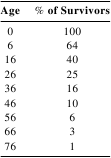
\includegraphics[scale=1.55]{InsuranceTable1.png}
%\begin{tabular}{@{}cc@{}}\toprule
%\textbf{Age} & \textbf{$\%$ of Survivors}\\\midrule
%$0$ & $100$\\
%$6$ & $64$\\
%$16$ & $40$\\
%$26$ & $25$\\
%$36$ & $16$\\
%$46$ & $10$\\
%$56$ & $6$\\
%$66$ & $3$\\
%$76$ & $1$\\\bottomrule
%\end{tabular}
\end{image}

\begin{question}
According to Graunt's London Life Table, what percentage of the population did not survive to age $16$?

\answer{60}$\%$
	
\end{question}

With the kind of information like that found in Graunt's table, a prospective insurer could answer questions like: How probable is it that a $16$-year old buying life-insurance now will die within the next $10$ years?

\begin{question}
According to Graunt's table, what percentage of $16$-year olds lived to be $26$-years old?

\begin{hint}
Out of $100$ people, how many lived to $16$? to $26$?
\end{hint}
\begin{hint}
What percentage of $40$ is $25$? 
\end{hint}
\begin{hint}
Don't round your answer.
\end{hint}
\answer{$62.5$}$\%$
	
\end{question}

Modern insurance companies collect and analyze a vast array of information so that they can make accurate predictions about the number and size of the claims they will face. Here is a small example where information is collected, analyzed, and the results used to sell insurance:

Phoebe's neighborhood has been plagued by bicycle thefts. As a result, some bicycle owners have bought bike locks and all are interested in insuring against theft. After conducting some research, Phoebe estimates that for every $40$ unlocked bicycles in the neighborhood, one is stolen each month, but only $1$ in $100$ locked bikes is stolen each month. Furthermore, Phoebe calculates the average value of the bicycles in her neighborhood at $\$200$ each.

Using the above data, and the fact that her neighborhood contains $300$ bicycles, half of which are unlocked, Phoebe creates the following table:

\begin{center}
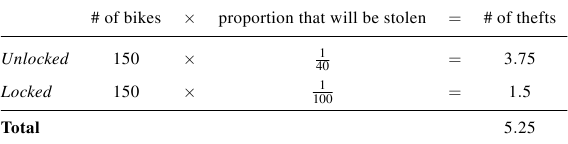
\includegraphics[scale=1.5]{InsuranceTable2.png}
%\renewcommand{\arraystretch}{2}
%\begin{tabular}{@{}lcccccc@{}}
% & \# of bikes & $\times$ & proportion that will be stolen & $=$ & \# of thefts\\\midrule
%\textit{Unlocked} & $150$ & $\times$ & $\frac{1}{40}$ & $=$  & $3.75$\\
%\textit{Locked} & $150$ & $\times$ & $\frac{1}{100}$ & $=$ & $1.5$\\\bottomrule
%\textbf{Total} & & & & & \textbf{$5.25$}
%\end{tabular}
\end{center}

An expectation of $5.25$ thefts corresponds to an expected loss in bicycle value of $5.25\times\$200=\$1,050$. Since $\$1,050\div 300=\$3.50$, Phoebe convinces each bike owner to pay her $\$5$ per month to insure their bike against theft. If Phoebe's calculations are close to accurate, then she stands to make a profit of $\$1,500-\$1,000=\$500$ if $5$ bikes are stolen and $\$1,500-\$1,200=\$300$ if $6$ bikes are stolen.

Of course, Phoebe could even more shrewdly charge those who leave their bikes unlocked more for insurance (a reasonable practice considering unlocked bikes are more likely to be stolen) and make an even larger profit.


\begin{question}
Suppose Phoebe charges owners of unlocked bicycles $\$7.50$ and owners of locked bicycles $\$3$ for insurance. How much would Phoebe earn if there were $6$ thefts that month?

\begin{hint}
How much will Phoebe collect in premiums from the owners of unlocked bicycles? How much from the owners of locked bicycles?
\end{hint}
\begin{hint}
How much will $6$ bicycle thefts cost Phoebe?
\end{hint}
\begin{hint}
Phoebe's profit is calculated by subtracting the cost of the claims she must pay from the premiums she collected.
\end{hint}
$\$$\answer{$375$}

\end{question}

We will revisit Phoebe's bicycle insuring business in class to see how she can become even more sure of turning a profit, but for now we are only interested in the general process of using estimated risk to help calculate a reasonable cost for insurance.
\end{document}
